\documentclass[11pt, letterpaper]{article}
\usepackage[utf8]{inputenc}
\usepackage{graphicx}
\usepackage{eso-pic}
\usepackage{soul}
\usepackage{xcolor}

\usepackage{fancyhdr}
% \usepackage{pagecounting}
% \usepackage[dvips]{color}

\newcommand{\illinoislogo}{
\includegraphics[height=0.5in]{images/illinoislogo.png}}
\newcommand{\anslogo}{\hspace{-4mm}
\includegraphics[height=0.5in]{images/ansuiuc.png}}
\newcommand{\anssite}{ans.npre.illinois.edu}
% \usepackage{background}
\usepackage{float}
\usepackage[top=2cm, bottom=2cm, outer=2cm, inner=2cm]{geometry}
\setcounter{tocdepth}{3}
% \setcounter{secnumdepth}{3}

\graphicspath{{./images/}}


% Creates the flow chart for conference management
\usepackage{tikz}
\usetikzlibrary{shapes.geometric, arrows}

\tikzstyle{chair} = [rectangle, rounded corners, minimum width=2cm, minimum height=1cm,text centered, draw=black, fill=blue!30]
\tikzstyle{director} = [rectangle, rounded corners, minimum width=2cm, minimum height=1cm,text centered, draw=black, fill=green!30]
\tikzstyle{coordinator} = [rectangle, rounded corners, minimum width=2cm, minimum height=1cm,text centered, draw=black, fill=red!30]
\tikzstyle{arrow} = [thick,->,>=stealth]


% \backgroundsetup{
% scale=1,
% angle=-90,
% opacity=.4,  %% adjust
% contents={\includegraphics[width=\paperwidth,height=\paperheight]{earth1.png}}
% }

\begin{document}

\begin{titlepage}
\AddToShipoutPictureBG*{\includegraphics[angle=90, width=\paperwidth,height=\paperheight]{earth1.png}};


   \begin{center}

       \vspace*{1cm}
 
       \Huge\color{white}\textbf{Saving the World One Atom at a Time}
 
       \vspace{0.5cm}
       Nuclear, Plasma, and Radiological Engineering
 
       \vspace{1.5cm}
 
       \Large\textbf{Presented by ANS at the University of Illinois Urbana-Champaign}
 
       \vfill
       \vspace{0.8cm}
 
       
\includegraphics[width=0.4\textwidth]{ans_sc_logo3.png}
   \end{center}
\end{titlepage}

\clearpage
\newpage

\pagestyle{fancy}
\lhead{\anslogo}
\rhead{\illinoislogo}

[Letter from the Chairs goes here!]

\newpage
\tableofcontents
\newpage


% ===============================================================================================
% ===============================================================================================
% ============================================THEME==============================================
% ===============================================================================================
% ===============================================================================================
\section{Saving the World One Atom at a Time}
There are many challenges facing the world today and some have been designated existential threats to humanity. Young people today will witness the growing toll of anthropogenic climate change. As students, obstacles at the scale of the world climate crisis appear daunting and overwhelming. We believe that many solutions will come from the nuclear sciences. The ANS student conference is an opportunity for students and professionals to come together and share advances in critical technology and research, dedicated to solving these problems. Whether the problem is solving the world’s energy needs, developing technology that will take us to the stars, or curing cancer, nuclear, plasma, and radiological engineering will be at the center of those endeavors. Our goal is to inspire and motivate students in nuclear, plasma, and radiological engineering fields to tackle big problems. Saving the world one atom at a time reflects the fact that nuclear science is a powerful force in dealing with grand challenge problems. This theme also honors the individual, atomic, contributions from students, researchers, and professionals, in the field of nuclear engineering, that are essential to progress. This conference is about science and it is about the people that make the science possible. Students will hear from visionary speakers and leaders of the nuclear science community and come away with optimism for the future; knowing that they are saving the world one atom at a time.\\
The University of Illinois at Urbana-Champaign chapter of ANS would be honored to host the 2021 student conference. We hope to create an atmosphere that will galvanize students and professionals for the exciting future of nuclear engineering.

% ===============================================================================================
% ===============================================================================================
% ========================================About UIUC=============================================
% ===============================================================================================
% ===============================================================================================

\newpage
\section{Champaign-Urbana and UIUC}
\subsection{About Champaign-Urbana}
Champaign-Urbana (CU) is a close-knit community filled with music, culture, and food. While Campustown, the neighborhood immediately surrounding campus,  is an important part of the atmosphere, there is plenty to do off campus. Relax in one of the outdoor restaurants downtown or walking through the various gardens and parks around town. The culture in Champaign is very rich as a result of many annual festivals such as the CU Pride Parade, the Ellnora guitar festival, and the Pygmalion festival. The Krannert Center for the Performing Arts is also a world-renowned theater that has hosted groups from all genres like the New York Philharmonic, the Russian National Ballet, and Sonny Rollins.

\subsubsection{Accessibility}
Myriad festivals and sporting events on campus draw many people to Champaign-Urbana at varying times of the year, which means hotels are not hard to find. A large number of these hotels are located around downtown Champaign and the Eastern side of campus, making transportation easy. There is also a small airport, Willard Airport, just 20 minutes from campus that regularly has flights to and from the Chicago O’Hare and Dallas Ft Worth airports. Finally, there are several reliable bus services that make frequent trips from Champaign-Urbana to O’Hare and the Chicagoland area.

\subsubsection{Weather}
With an average high temperature of 65$^\circ$F and an average low temperature of 40$^\circ$F , April in Champaign is a gorgeous month of dwindling winter weather as summer begins to round the corner. Hlding a conference during this time would be the perfect way to showcase our beautiful city.

\subsection{About the University of Illinois}
Founded in 1867, the University of Illinois at Urbana-Champaign (UIUC) has cultivated a long history of significant scientific discoveries and contributions. The theory of superconductivity, the invention of the transistor, the discovery of archaea, the fourth domain of life, and the first web browser are just some of the many breakthroughs from UIUC. Established in 1876, the famous Morrow Plots became the first research crop field at a university and is still used today. Attendees will also be familiar with Blue Waters, one of the world’s fastest supercomputers. 
The UIUC Grainger College of Engineering has had sixteen Nobel Laureates in physics. Including John Bardeen, the only scientist to ever win the award twice. It also offers 15 different majors to more than 9,100 undergraduate and 3,400 graduate students. Of its twelve ranked majors, nine are ranked among the top 10 in the nation, and six of which remain ranked among the top 5 in their degree. Overall, the College of Engineering in Urbana-Champaign ranks sixth among the nation’s best undergraduate engineering programs. With more than 250 degrees for undergraduates and graduates and a multitude of first-class research facilities and resource, UIUC gives its 45,000 students the ability to succeed.\\
Today, the University of Illinois at Urbana-Champaign attracts visitors from throughout the state by offering a variety of valuable public attractions. UIUC maintains four public museums: the Spurlock Museum, containing 54,000 cultural artifacts from around the world; the Illinois Natural History Survey, has more than 9.5 million biologic specimens in its collection; the Sousa Archives and Center for American Music, provides shows and education to students and the public; and the Krannert Art Museum, offers fine arts and education. More than 470,000 square feet of recreational space is occupied by other facilities including an ice arena, climbing wall, swimming pools, parks, sports fields, parks, and outdoor adventure venues. 

\subsection{UIUC ANS Student Chapter (ANS-UIUC)}
The ANS-UIUC maintains and develops a cohesive community of students in nuclear, plasma, and radiological engineering (NPRE). It also engages in education and outreach programs to teach members of the surrounding community about nuclear science. Membership is currently around 70-80 students and has been steadily growing. The chapter works to host events catering to nuclear, plasma, and radiological concentrations. It also makes professional development a large part of member involvement. ANS-UIUC has historically been one of the best represented institutions at the annual student conference and is a tradition this chapter is eager to uphold. 

% Group picture from the 2019 kick off barbeque.
\begin{figure}[H]
  \centering
  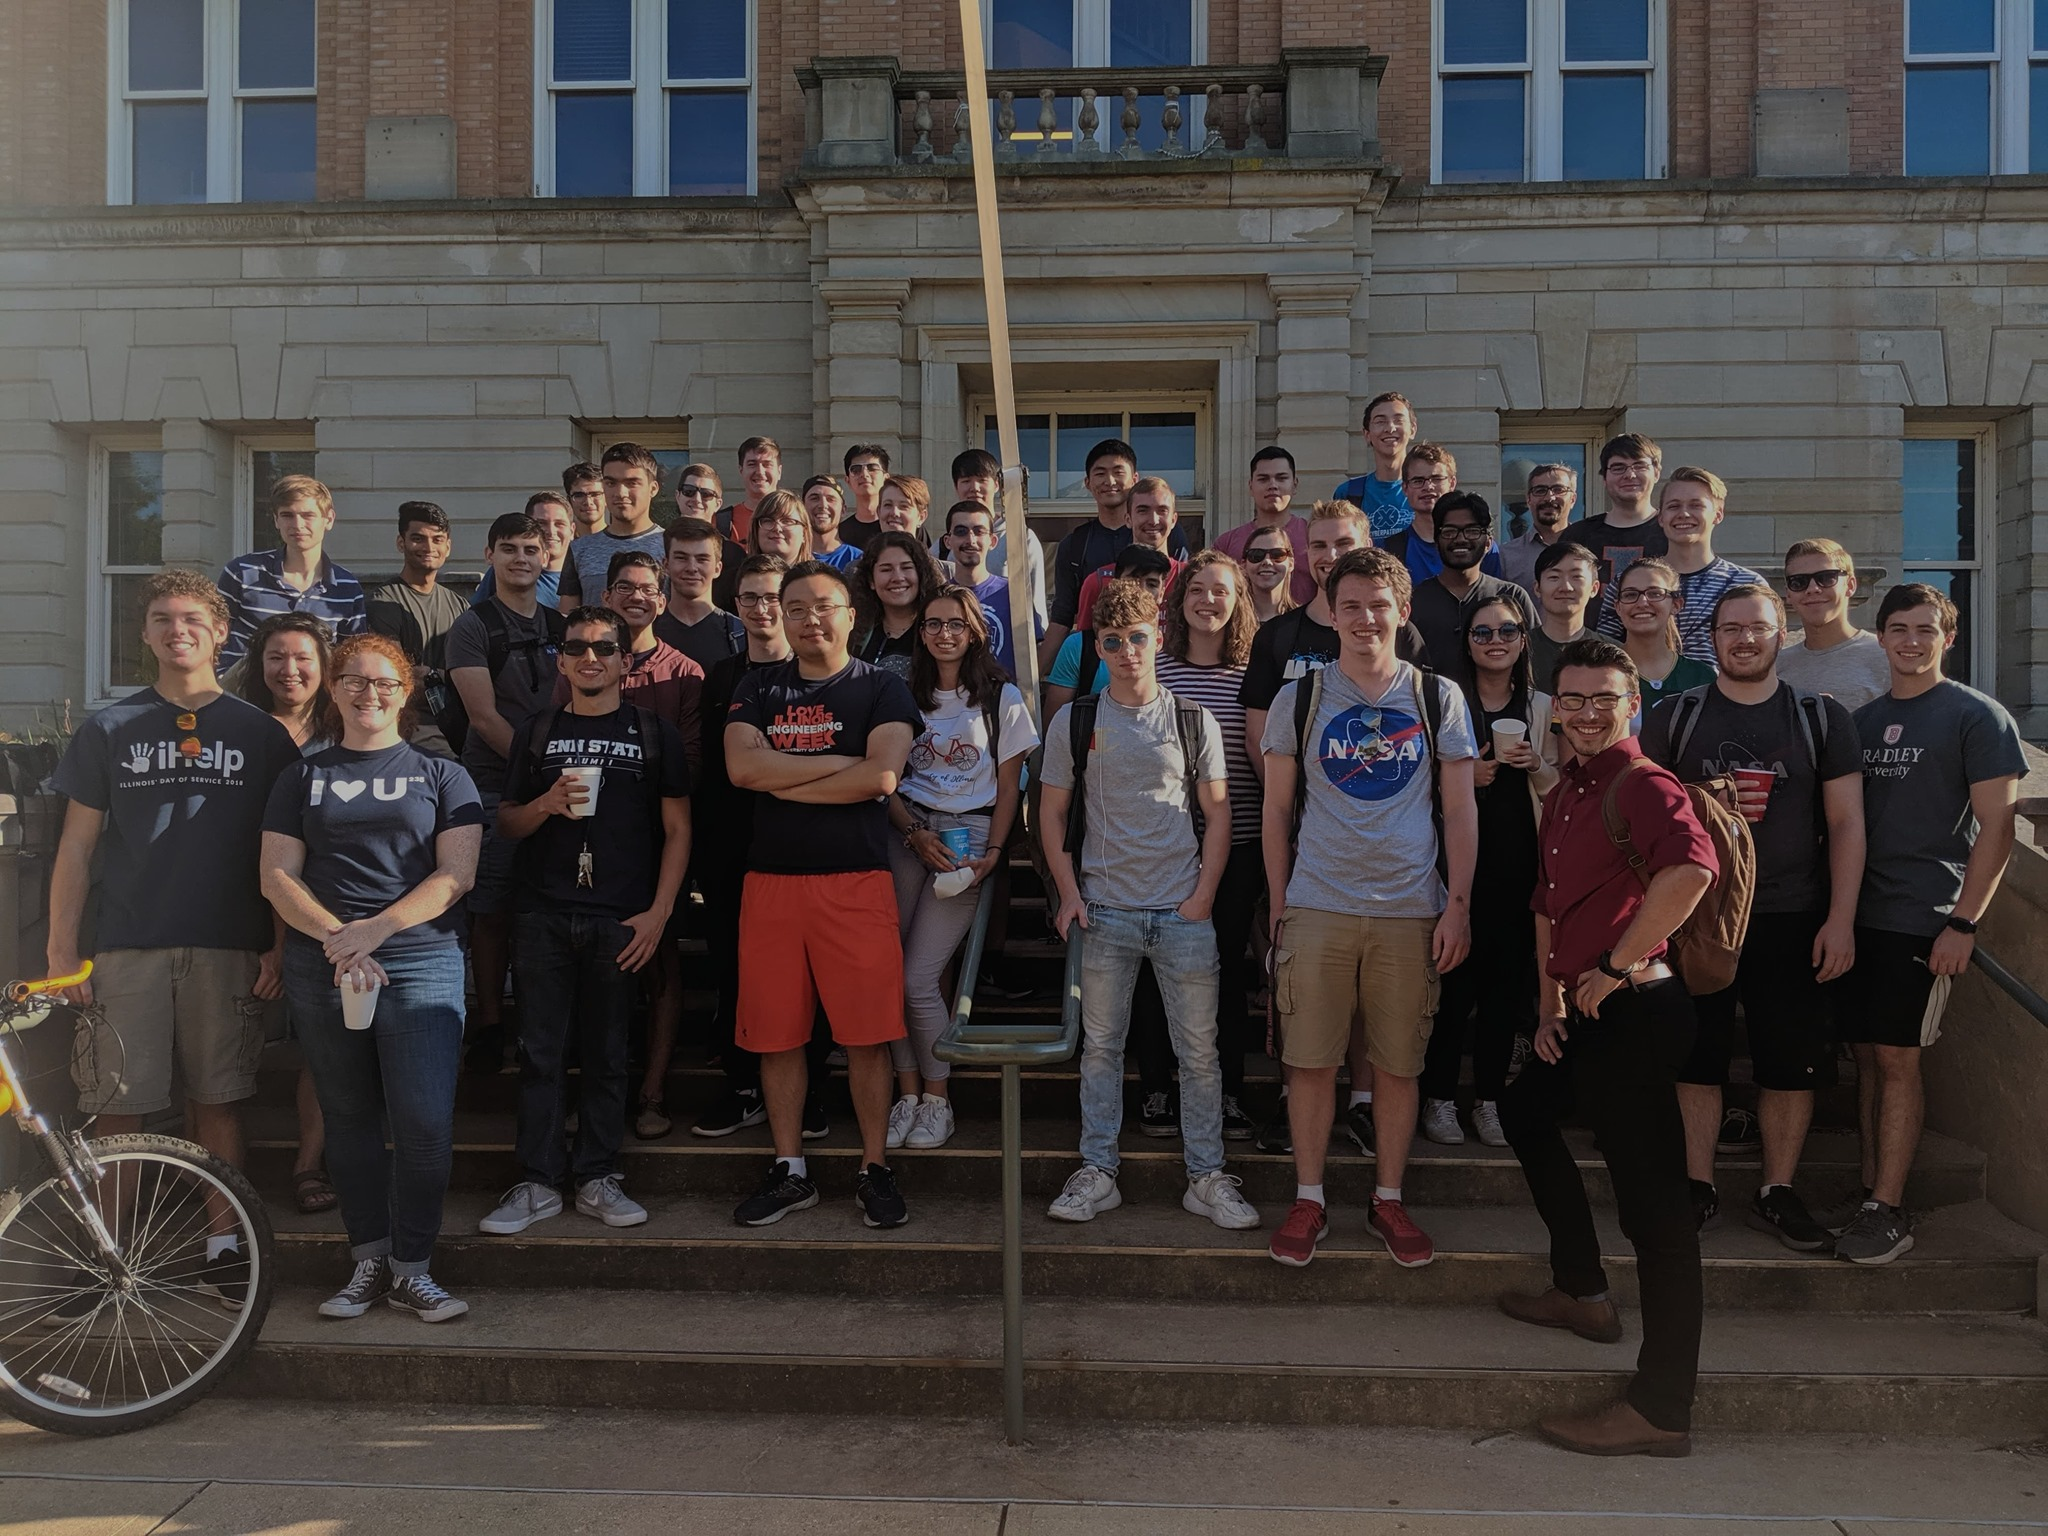
\includegraphics[width=12cm]{ans_uiuc_group.jpg}
  \caption{Members of ANS-UIUC at the 2019 Kick Off Barbeque.}
\end{figure}

% Picture of attendees to the 2019 ANS Student Conference
\begin{figure}[H]
  \centering
  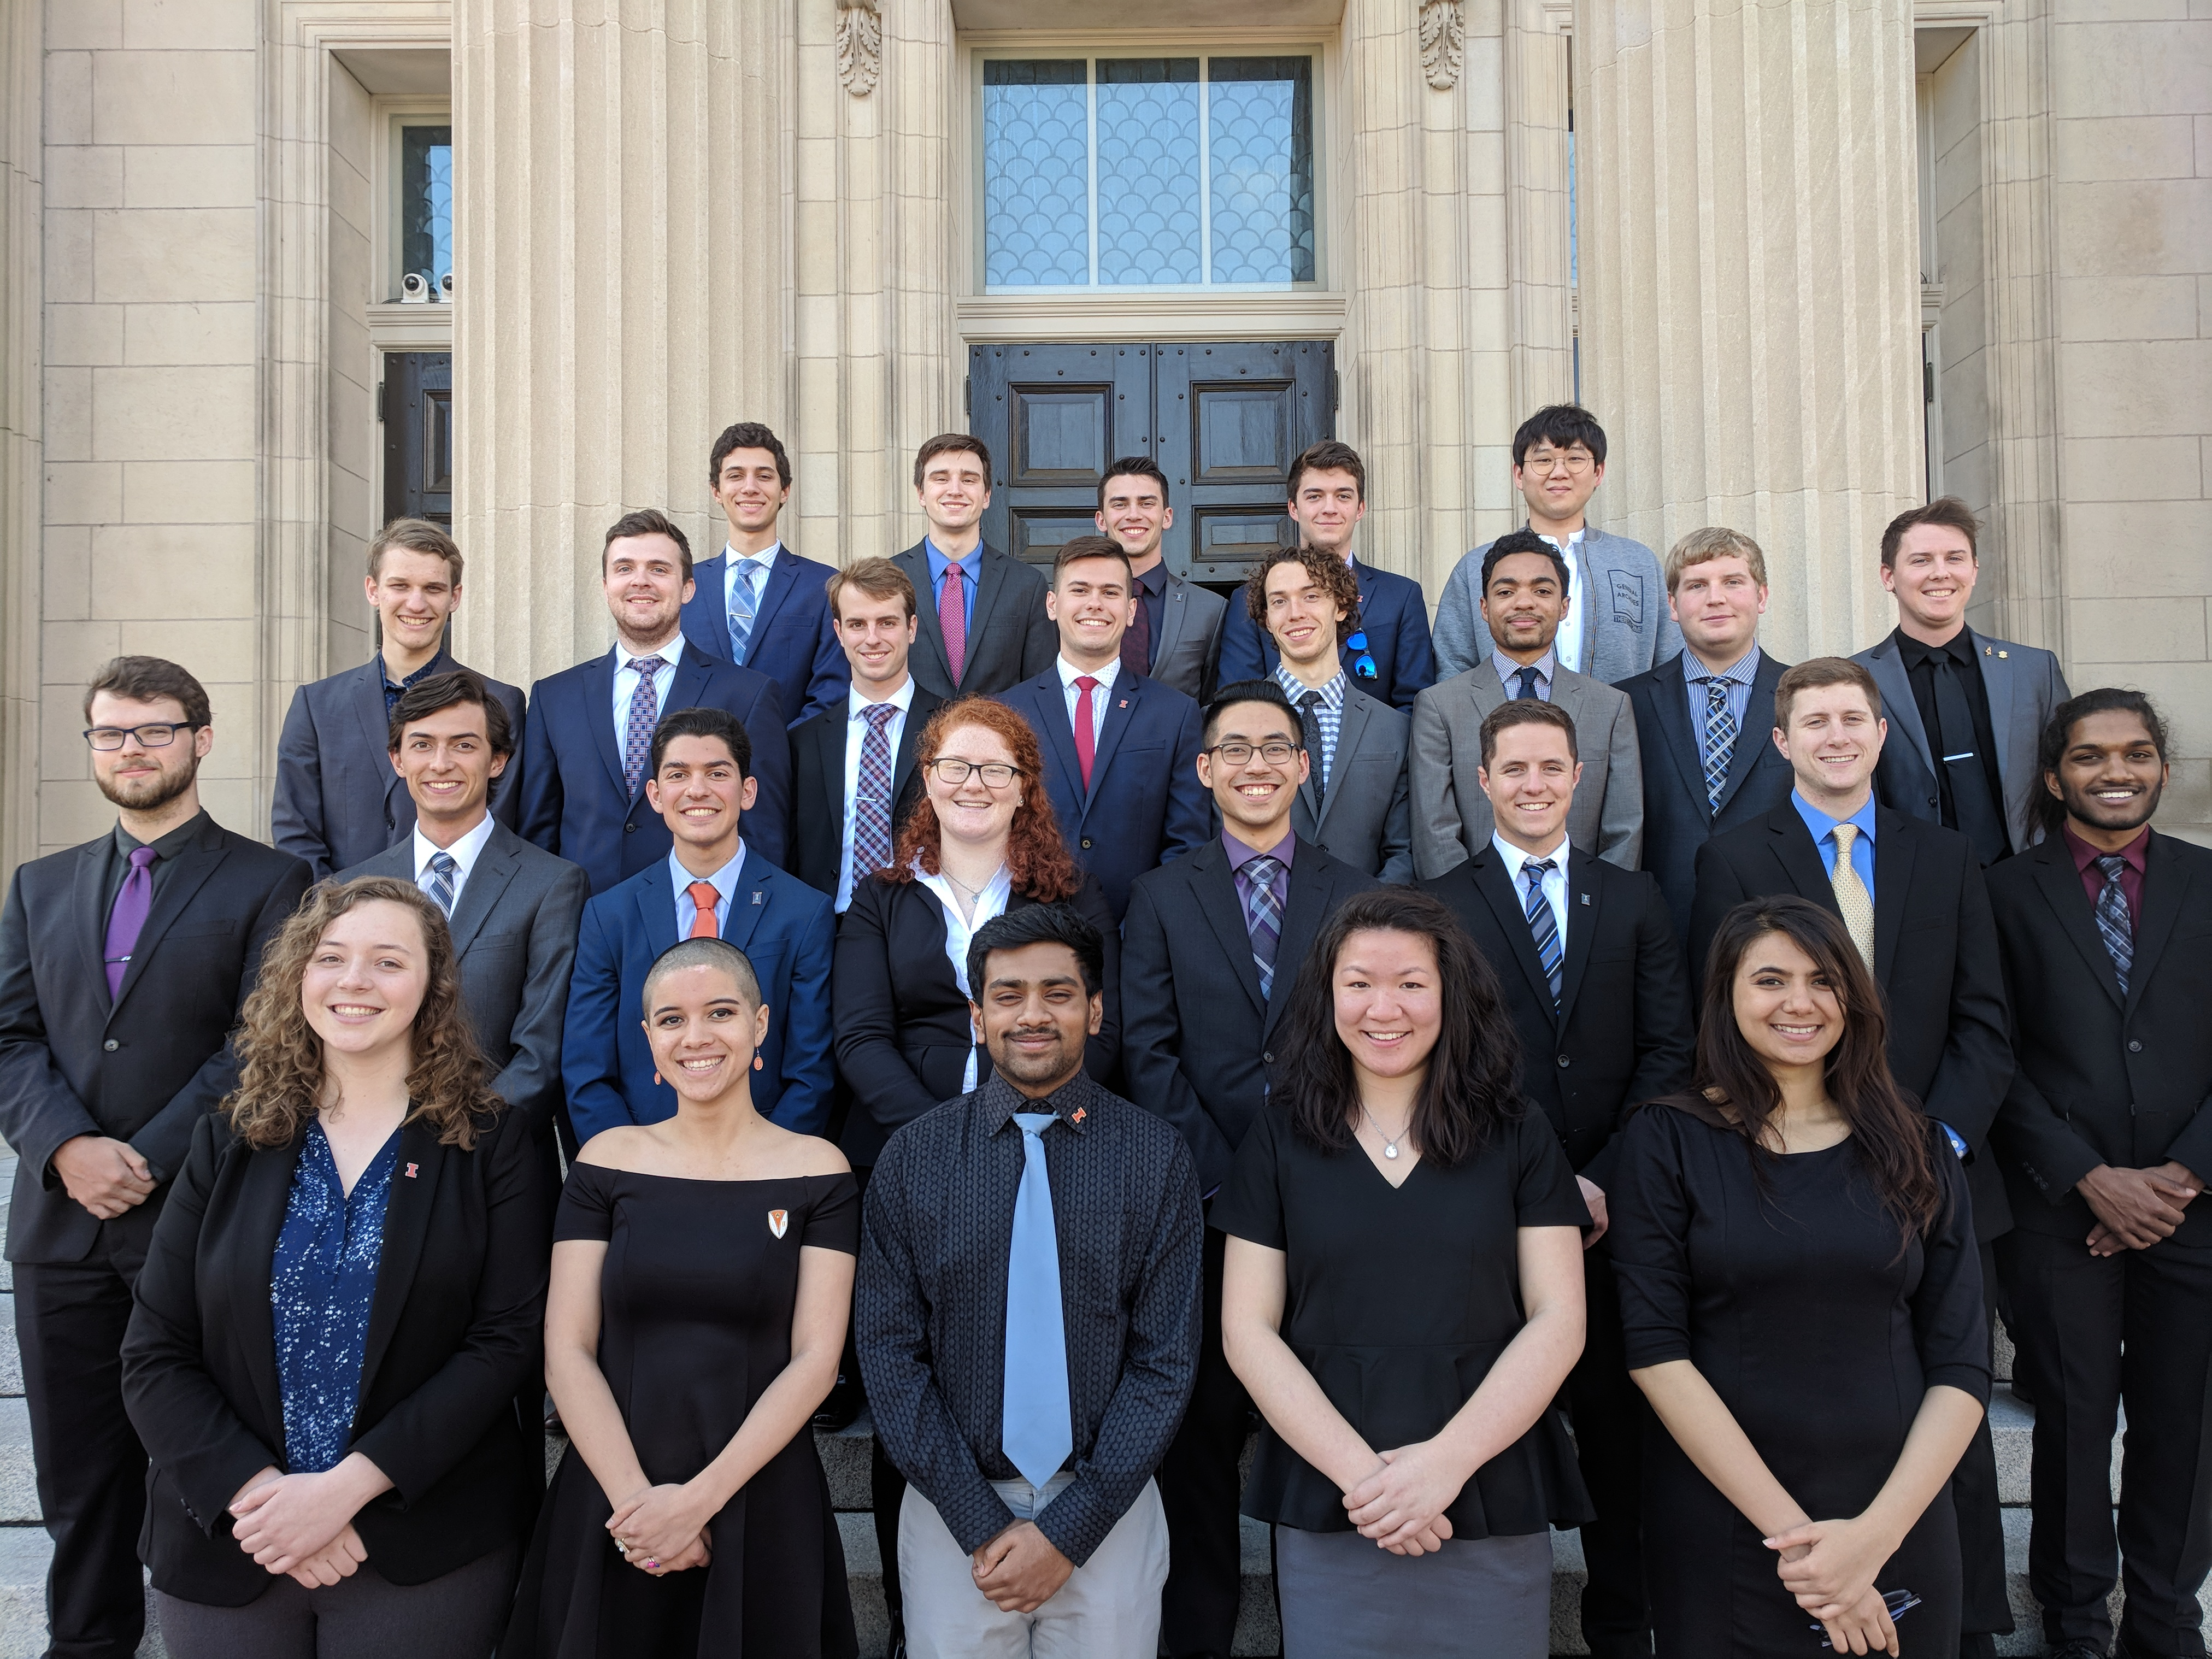
\includegraphics[width=12cm]{ans_conf_19.jpg}
  \caption{Members of ANS-UIUC at the 2019 Student Conference at VCU.}
\end{figure}

\subsection{Research at UIUC}
Faculty in NPRE conduct research in many areas of interest to the nuclear science community. Students are highly encouraged to participate and make their own atomic contributions that will someday save the world.

\subsubsection{Nuclear Power}
The Department of Nuclear, Plasma, and Radiological Engineering at Illinois is well known for its pioneering research in the area of reactor power engineering. Graduates have gone on to leadership positions in industry, national laboratories, and academia. Research in the Nuclear Power concentration covers all aspects of power generation using nuclear energy on land, underwater (submarine), and in space. It is inherently interdisciplinary and relies on several branches of physics and engineering for design and analysis of large complex systems. These include aspects of reactor physics, reactor thermal-hydraulics, reactor safety, reliability and risk, instrumentation and control, training and education, human factors engineering, reactor materials, nonproliferation, and more. Safety starndards and maintenance for existing reactors and new reactor designs are also explored by faculty in the department. Cross-cutting areas of research include multi-physics and multi-scale modeling and simulation, high performance computing, reliability and risk, validation and verification, and uncertainty analysis. Recently, the University of Illinois declared a plan to be completely carbon-neutral by 2050. Nuclear power is the perfect candidate to help UIUC attain its energy goals. Together, the University and the NPRE department are saving the world one atom at at time.

\subsubsection{Plasma Physics and Fusion Science}
The research theme of Fusion and Plasma Physics in the NPRE department has a long history of work in the area of magnetic and inertial nuclear fusion as well as plasma engineering. NPRE is now one of the leading departments in plasma-material interactions with its Center for Plasma-Materials Interactions established by Prof. David Ruzic. Furthermore, in the past few years, three new faculty members have been added to this area including: Prof. Davide Curelli and Prof. Daniel Andruzcyk. There are five research themes that spans the work in fusion and plasma physics: fusion materials, plasma-material interface (PMI) diagnostics, plasma-edge and PMI modeling, plasma nanosynthesis, and plasma sources and processing. The Hybrid Illinois Device for Research and Application (right) marks the newest addition to the team at CPMI. This device finished construction and achieved first plasma during the spring of 2016

\subsubsection{Radiological Science}
Radiological engineering at UIUC strives to discover novel applications for ionizing radiation in biomedical research, homeland security, and nuclear safeguards. We have developed various gamma-ray, x-ray and neutron detectors, imaging devices, and novel algorithms for analyzing the data from these systems. These algorithms range from the use of so-called "big data" techniques applied to large sensor networks to advanced radiological imaging methods and image processing techniques for biomedical research. We work with physicists, biologist, chemists, material scientists, statisticians, and physicians around the world, to develop advanced diagnostic imaging and radiation-induced therapeutic approaches to address some of the most critical health care-related issues, such as cancer, cardiac diseases, diabetes and neurodegenerative disorders. We also work with organizations like the Departments of Defense, Energy, and Homeland Security and the International Atomic Energy Agency to deploy our research around the world to detect and identify the illicit movement of nuclear and radiological materials.

\subsubsection{Reliability and Risk Analysis}
Risk analysis represents the pinnacle of interdisciplinary research and education. Following the Three Mile Island disaster in 1979, Probabilistic Risk Assessment (PRA) has become a key pillar of the risk-informed nuclear regulatory framework, and is now a requirement for every nuclear power plant in the United States. Enhancing the prevention of catastrophic technological accidents and the protection of the environment requires advancement in multidisciplinary PRA. It demands the development of a common vocabulary within diverse engineering and social science domains in order to address risks emerging from the interface of social and technical systems.


\subsubsection{Materials Science}

\subsubsection{NPRE Research Groups and Laboratories}
\begin{itemize}
  \item \textbf{Advanced Reactors and Fuel Cycles (ARFC)} - \textit{Dr. Katy Huff}\\
  The ARFC group seeks to advance the safety and sustainability of nuclear energy production through improved reactor designs, fuel cycle strategies, and waste management techniques. In the area of advanced reactors, our work focuses on extending current simulation tools with features essential to advanced reactor multiphysics. In the context of the broader nuclear fuel cycle, the ARFC group emphasizes modeling, simulation, and analysis of the global nuclear fuel cycle, with an emphasis on sustainability. A crosscutting theme of our research is an emphasis on advancing methods and software for computational nuclear engineering. Accordingly, the Advanced Reactors and Fuel Cycles group is proud to be affiliated with the University of Illinois National Center for Supercomputing Applications and its Blue Waters computing facility.
  \item \textbf{Virtual Education and Research Laboratory (VERL)} - \textit{Dr. Rizwan Uddin}\\
  The VERL group focuses on the development of innovative numerical methods and their implementation on high performance computing machines. Research efforts center on problems in nuclear engineering, with emphasis on thermal-hydraulics and reactor physics.

  \item \textbf{Analysis of Reactor Transients and Stability (ARTS)} - \textit{Dr. Tomasz Kozlowski}\\
  The ARTS group performs deterministic safety analysis by developing and validating advanced methods to accurately determine reactor safety margins and reactor behavior. By performing high-fidelity numerical predictions of the reactor behavior in abnormal transient scenarios of safety significance, our work supports the nuclear reactor safety analysis, and increases the fidelity of primary system simulation. This approach is at the heart of nuclear power’s excellent safety record – always striving to improve current tools and methods.

  \item \textbf{Center for Plasma-Material Interactions (CPMI)} - \textit{Dr. David Ruzic}\\
  The primary objective of CPMI is the study of plasma-material interactions relevant to fusion, semiconductor manufacturing, and plasma processing through a combination of experimental and computational means. CPMI has facilities for the study of fusion materials, High Power Impulse Magnetron Sputtering (HiPIMS), liquid metals, Extreme Ultraviolet Lithography (EUVL),  laser-material interactions, and more. Projects are supported by both government and commercial partners to further the application and knowledge of plasma physics. The facility recently finished the construction of the HIDRA fusion device, which is a stellarator-tokamak machine hybrid machine used to study plasma-materials interactions.  HIDRA is currently run by Dr. Daniel Andruczyk.

  \item \textbf{Materials Science} - \textit{Dr. James F. Stubbins}\\
  The group investigates a wide variety of topics within the realm of materials research including mechanical properties, microstructural evaluations, plus radiation damage investigations, and modeling. Materials such as copper alloys nickel-based alloys, stainless steels, ferritic steels, and silicon-carbide composites are studied using a variety of analytical techniques electron microscopy and spectroscopy.


  \item \textbf{Non-Equilibrium Matter Laboratory} - \textit{Dr. Yang Zhang}\\
  This laboratory focuses on the study of non-equilibrium matter, with particular emphasis on liquids and soft matter, using integrated neutron and synchrotron light experimental probes and atomistic modeling and simulation. The structure and dynamics of these systems are either inherently complex or driven away from equilibrium by extreme conditions. In particular, our current interests include a range of fundamental and technical problems involving slow phenomena and rare events, such as: materials far from equilibrium and in extreme environments; extreme properties of liquids; and glassy or jammed soft matters.

  \item \textbf{Radiation Imaging Group} - \textit{Dr. Ling Jian Meng}\\
  Research is on developing radiation sensor and systems for visualizing the distribution of radioactivity in surrounding objects, patients, and small lab animals etc. Current emphasis includes (a) developing novel radiation sensors for detecting X-ray, gamma rays and neutrons, and (b) developing nuclear techniques for detecting and imaging a tiny amount radiolabeled molecules inside small lab animals.

  \item \textbf{Socio-Technical Risk Analysis (SoTeRiA)} - \textit{Dr. Zahra Mohaghegh}\\
  The Socio-Technical Risk Analysis (SoTeRiA) Laboratory is evolving Probabilistic Risk Assessment (PRA) by explicitly incorporating the underlying science of accident causation into risk scenarios. SoTeRiA laboratory has pioneered two key areas of theoretical and methodological innovations: (1) spatio-temporal causal modeling of social and physical failure mechanisms in PRA, and (2) the fusion of big data analytics with PRA. The Lab’s current projects include: Fire PRA; Location-specific Loss- Of-Coolant Accident (LOCA) Frequency Estimations; Risk-Informed Resolution of Generic Safety Issue 191; Human and Organizational Influences on System Risk; Risk-Informed Regulation; and Risk-Informed Emergency Preparedness, Planning and Response.

  \item \textbf{Laboratory: High Temperature Environmental Exposure Lab} - \textit{Dr. Brent Heuser}\\
  A simultaneous thermal analyzer with combined thermogravimetric and differential scanning calorimetry function is housed in this laboratory. The response of LWR fuel cladding materials in high temperature steam environments for improved accident tolerance is currently of interest.

  \item \textbf{Laboratory: Nuclear Materials Fabrication and Studies Lab} - \textit{Dr. Brent Heuser}\\
  The Radiation Detection and Imaging Lab focuses on developing non-invasive imaging technology for use in preclinical medical research. Many of our current endeavors focus on developing semiconductor Single Photon Emission Computed Tomography (SPECT) and Positron Emission Tomography (PET). These works challenge the current state of the art for spatial resolution and system sensitivity. The use of highly pixelated CdTe detectors has driven our work to break into a spatial resolution on the order of 300 microns for both PET and SPECT. Our work in SPECT has also challenged the limits of aperture sensitivity through the engineering of the compound-eye aperture.
\end{itemize}
% ===============================================================================================
% ===============================================================================================
% =====================================Conference Logistics======================================
% ===============================================================================================
% ===============================================================================================

\newpage
\section{Conference Logistics}

\subsection{Date Selection}
We are aware that there is no perfect date in which everyone who wants to attend the conference can do so. However, our hope is to accommodate as many students as possible with a proposed date of either: Thursday April 8th - Saturday April 10th or Thursday April 15th - April 17th, 2021. Two dates are proposed because the Mom's association that runs Mom's Weekend, one of the largest events of the year, has not announced their 2021 dates yet. Mom's weekend is typically held the first weekend of April which conflicts with Easter in 2021. This consensus was reached after looking up any holidays, scheduled spring breaks, final exams, and other miscellaneous conflict dates for 42 schools with active ANS student sections. Based on these findings, there are no major conflicts with any of the schools for these dates. These factors were considered in order to maximize the possible number of attendees that can benefit from the conference. A handful of schools did not have an academic calendar available for the 2021 Spring semester, so data was based on their listed 2020 dates. These date selections avoid conflicting with large event weekends such as Mom's Weekend, dates pending, and the Illini Marathon. If, for some reason, an issue arises with our proposed dates, our back-up date is Thursday April 1st - Saturday April 3rd. This is unfortunately the same weekend as Easter Sunday. However, we prioritized avoid final exams, and UIUC’s Mom’s Weekend. Please see the appendix for the full conflicts calendar.

\subsection{Conference Facilities}
\begin{itemize}
  \item \textbf{The Illini Union}\\
  \item \textbf{National Center for Supercomputing Applications (NCSA)}\\
  \item \textbf{Engineering Hall}\\
  \item \textbf{The I-Hotel}\\
  \item \textbf{}\\
\end{itemize}


\subsection{Facilities Contingency Plan}
Words

% ===============================================================================================
% ===============================================================================================
% ======================================Program Logistics========================================
% ===============================================================================================
% ===============================================================================================
\newpage
\section{Program Logistics}

% ===============================================================================================
% ===============================================================================================
% ====================================Conference Management======================================
% ===============================================================================================
% ===============================================================================================
\newpage
\section{Conference Management}

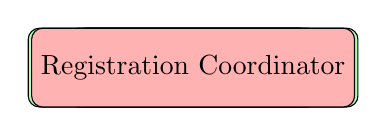
\begin{tikzpicture}[node distance = 2cm] 
  
  \node (gen chair) [chair] {General Co-Chair};
  \node (tech chair) [chair] {Technical Co-Chair};
  \node (fin dir) [director] {Financial Director};
  \node (pub dir) [director] {Communications Director};
  \node (reg coord) [coordinator] {Registration Coordinator};
  % \node (gen chair) [chair] {General Co-Chair};
  % \node (gen chair) [chair] {General Co-Chair};
  % \node (gen chair) [chair] {General Co-Chair};
  % \node (gen chair) [chair] {General Co-Chair};
  % \node (gen chair) [chair] {General Co-Chair};

\end{tikzpicture} 

% ===============================================================================================
% ===============================================================================================
% ======================================Conference Budget========================================
% ===============================================================================================
% ===============================================================================================

\newpage
\section{Conference Budget}


\end{document}
